%%%%%%%% ICML 2026 PAPER: Dynamic Tokenization for Chemical SMILES %%%%%%%%%%%%%%%%%

\documentclass{article}

% Recommended packages
\usepackage{microtype}
\usepackage{graphicx}
\usepackage{subcaption}
\usepackage{booktabs}
\usepackage{hyperref}
\usepackage{xcolor}

% Attempt to make hyperref and algorithmic work together better:
\newcommand{\theHalgorithm}{\arabic{algorithm}}

% Use for initial blind version submitted for review:
\usepackage{icml2026}

\usepackage{amsmath}
\usepackage{amssymb}
\usepackage{mathtools}
\usepackage{amsthm}

% Cleveref for referencing
\usepackage[capitalize,noabbrev]{cleveref}

% Custom commands
\newcommand{\hnet}{H-Net}
\newcommand{\smilespe}{SmilesPE}
\newcommand{\bpb}{BPB}
\newcommand{\ppl}{PPL}

% Running title
\icmltitlerunning{Learning Chemical Grammar: Dynamic Tokenization for SMILES}

\begin{document}

\twocolumn[
  \icmltitle{Learning Chemical Grammar: Dynamic Tokenization for SMILES \\ with Hierarchical Networks}

  \begin{icmlauthorlist}
    \icmlauthor{Anonymous Author(s)}{anon}
  \end{icmlauthorlist}

  \icmlaffiliation{anon}{Anonymous Institution}

  \icmlcorrespondingauthor{Anonymous Author(s)}{anonymous@example.org}

  \icmlkeywords{Chemical Language Models, Tokenization, SMILES, Molecular Representation, Foundation Models}

  \vskip 0.3in
]

\printAffiliationsAndNotice{}

\begin{abstract}
Tokenization fundamentally shapes how machine learning models represent chemical structures. While static tokenizers like SMILES Pair Encoding use predefined subword vocabularies, we investigate \emph{dynamic tokenization} using Hierarchical Networks (\hnet{}), which learn byte-level chunking patterns directly from data. We train 350M-parameter \hnet{} models on polymeric (PI1M) and molecular (MOSES) SMILES datasets, systematically analyzing how dataset nature, training context, training duration, and architecture affect learned tokenization. Our study reveals three key findings: (1)~\textbf{Dataset specificity matters}---\hnet{} learns distinct ``chemical vocabularies'' with only 30\% token overlap between polymer and molecular datasets, analogous to language-specific patterns in NLP; (2)~\textbf{Dynamic tokenization improves with training}---extended training yields 63\% more unique tokens and 23\% higher efficiency, achieving bits-per-byte of 0.64; (3)~\textbf{Learned representations transfer}---\hnet{} embeddings outperform RDKit descriptors on blood-brain barrier penetration classification (AUC 0.95 vs.\ 0.93) and achieve competitive polymer glass transition temperature prediction. We establish dynamic tokenization as a promising paradigm for chemical representation learning.
\end{abstract}

%%%%%%%%%%%%%%%%%%%%%%%%%%%%%%%%%%%%%%%%%%%%%%%%%%%%%%%%%%%%%%%%%%%%%%%%%%%%%%%
\section{Introduction}
\label{sec:intro}
%%%%%%%%%%%%%%%%%%%%%%%%%%%%%%%%%%%%%%%%%%%%%%%%%%%%%%%%%%%%%%%%%%%%%%%%%%%%%%%

Chemical machine learning relies on string-based molecular representations, with SMILES (Simplified Molecular Input Line Entry System)~\citep{weininger1988smiles} serving as the dominant format. However, the \emph{tokenization} of these chemical strings---how they are segmented into discrete units for model consumption---fundamentally constrains what patterns models can learn.

Current approaches employ \emph{static} tokenization strategies. Character-level tokenization treats each symbol independently, losing chemical semantics. Atom-level tokenization preserves chemical meaning through fixed vocabularies but cannot adapt to domain-specific patterns. Subword methods like \smilespe{}~\citep{li2020smilespe} apply BPE-style algorithms trained on large chemical corpora, achieving good compression while maintaining some chemical interpretability. Despite their differences, all these methods impose uniform tokenization regardless of the specific chemical domain---the same tokens are used for drug-like molecules, ionic liquids, or polymers.

This uniform approach may be suboptimal. In natural language processing, models trained on multilingual data learn language-specific tokenization patterns; Mandarin and English text yield fundamentally different token distributions even with shared architectures~\citep{hwang2025hnet}. We hypothesize that chemistry exhibits analogous domain specificity: polymeric structures, with their repeating units and larger sequence lengths, may benefit from different tokenization than small drug-like molecules.

To investigate this hypothesis, we apply \emph{dynamic tokenization} using Hierarchical Networks (\hnet{})~\citep{hwang2025hnet}, which learn byte-level chunking patterns directly from data through differentiable boundary prediction. Originally developed as a foundational architecture for natural language processing, \hnet{} demonstrated that end-to-end learned tokenization can match or exceed hand-designed subword methods across multiple languages. We adapt this architecture and its core principles to the chemical language domain. Unlike static tokenizers, \hnet{} adapts its tokenization to dataset characteristics, potentially discovering domain-specific chemical ``grammars.'' This approach aligns with Sutton's ``Bitter Lesson''~\citep{sutton2019bitter}: the strongest long-term gains in AI come from methods that leverage computation and data rather than relying on handcrafted components. By learning tokenization end-to-end, we remove a key hand-designed element from chemical language modeling.

\textbf{Contributions.} We present the first systematic study of dynamic tokenization for chemical SMILES strings. First, we train and analyze 8 \hnet{} models (350M parameters each) on polymeric and molecular datasets, systematically varying dataset nature, concatenation strategy, training duration, and architecture (both 1-stage and 2-stage hierarchical variants). Second, we develop a comprehensive metrics suite including token statistics, Jaccard similarity, KL divergence, breakpoint analysis, and bits-per-byte compression to characterize tokenization behavior. Third, we demonstrate that \hnet{} learns dataset-specific vocabularies with only 30\% token overlap between polymer and molecular domains---analogous to the divergence between languages in NLP. Finally, we validate that \hnet{} embeddings serve as effective chemical featurizers, outperforming RDKit descriptors on classification tasks including blood-brain barrier penetration (AUC 0.95 vs.\ 0.93) and HIV inhibition prediction (AUC 0.79 vs.\ 0.76).

\begin{figure}[t]
\vskip 0.1in
\begin{center}
\centerline{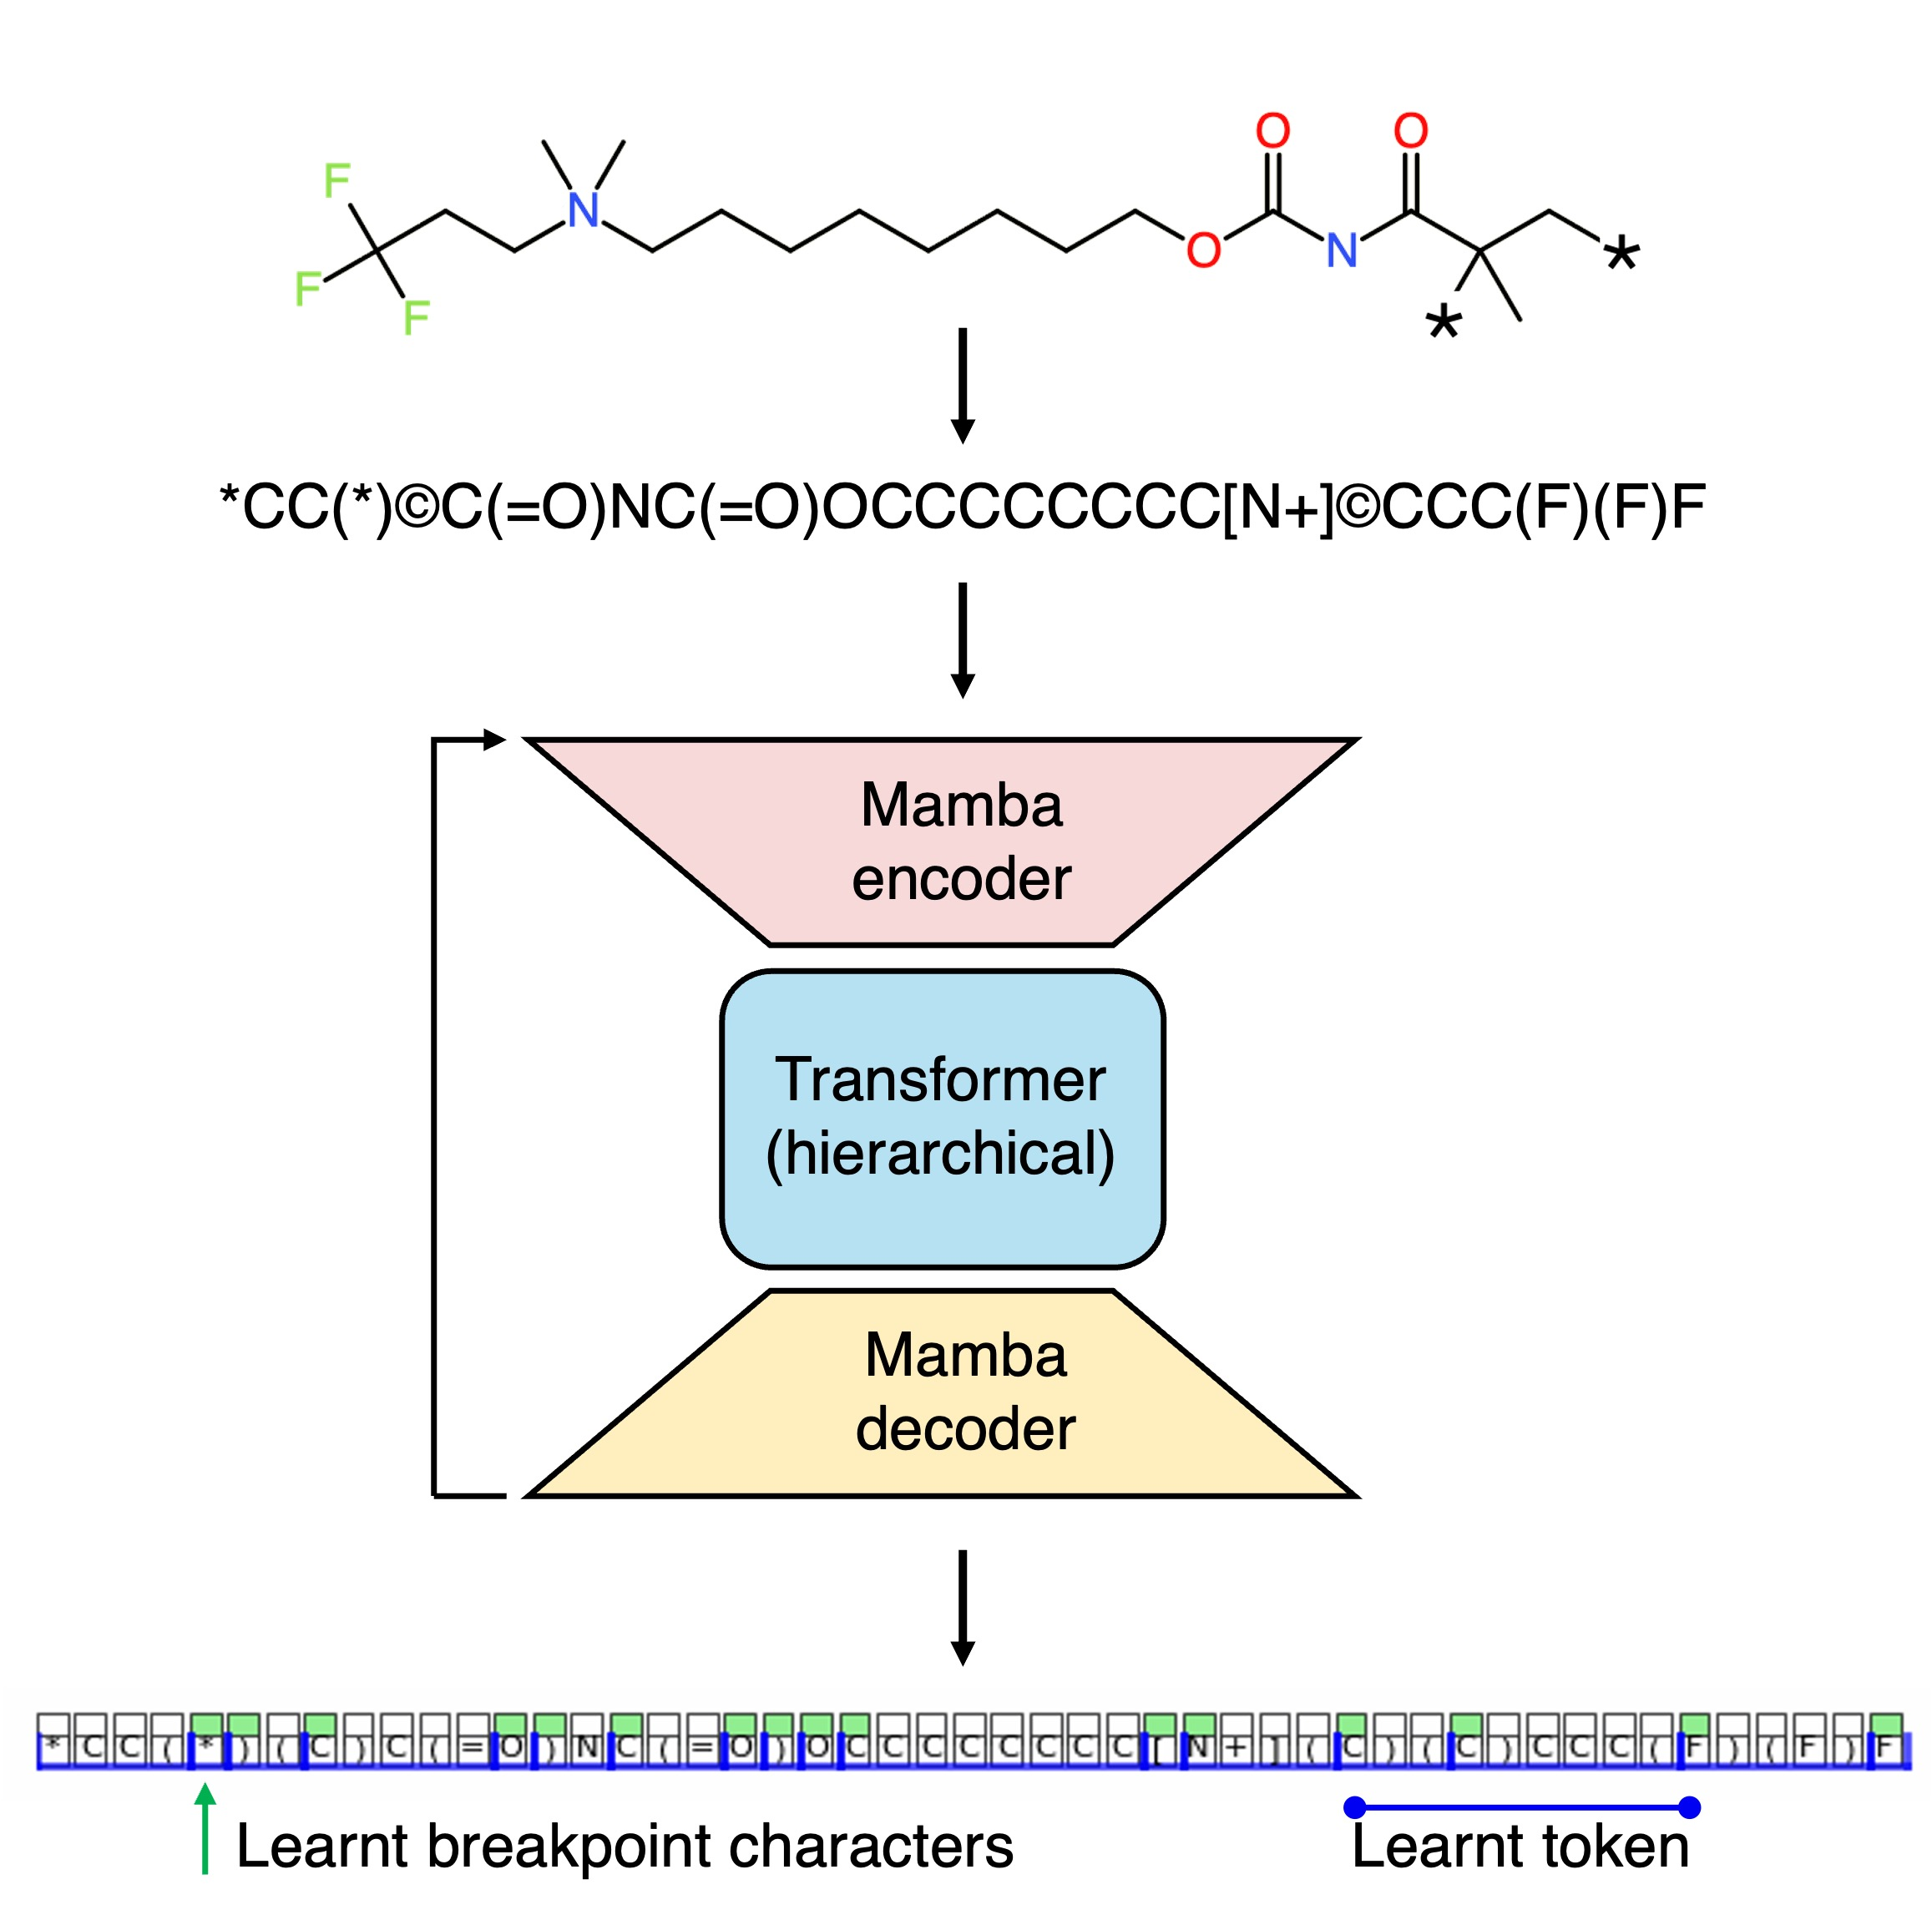
\includegraphics[width=\columnwidth]{figures/tokenization_schematic}}
\caption{H-Net dynamic tokenization pipeline for chemical structures. A chemical molecule (top) is converted into a SMILES-like string representation, which is then processed through the Mamba-Transformer-Mamba architecture: raw bytes enter a Mamba encoder, hierarchical boundary predictions are learned in Transformer layers, and tokens are decoded through a Mamba decoder. The output (bottom) shows tokenized segments with learnt breakpoint characters (highlighted in green) and learnt tokens (spanning multiple characters, shown in blue). Unlike static tokenizers, H-Net discovers chemically-meaningful segmentation patterns directly from data.}
\label{fig:tokenization_schematic}
\end{center}
\vskip -0.2in
\end{figure}

%%%%%%%%%%%%%%%%%%%%%%%%%%%%%%%%%%%%%%%%%%%%%%%%%%%%%%%%%%%%%%%%%%%%%%%%%%%%%%%
\section{Related Work}
\label{sec:related}
%%%%%%%%%%%%%%%%%%%%%%%%%%%%%%%%%%%%%%%%%%%%%%%%%%%%%%%%%%%%%%%%%%%%%%%%%%%%%%%

\textbf{Chemical String Representations.}
SMILES~\citep{weininger1988smiles} and its derivatives---SELFIES~\citep{krenn2020selfies} for guaranteed validity and PSMILES~\citep{audus2021psmiles} for polymer repeat units---provide the string-based inputs to chemical language models. Our work focuses on how these strings are tokenized rather than the representation format itself.

\textbf{Chemical Tokenization.}
Character-level tokenization is simple but ignores chemical structure. Atom-level methods preserve chemical meaning but use fixed vocabularies. \smilespe{}~\citep{li2020smilespe} applies pair encoding to learn subword vocabularies from ChEMBL, achieving good compression while maintaining chemical interpretability. However, all these approaches are \emph{static}---they produce identical tokenization regardless of the downstream dataset or task.

\textbf{Learned Tokenization.}
\hnet{}~\citep{hwang2025hnet} introduces hierarchical networks with learned dynamic chunking, demonstrating that byte-level models can learn optimal segmentation directly from data. Originally developed for natural language, \hnet{} showed that different languages induce different tokenization patterns. Byte-level transformers~\citep{wang2022blt} and patch-based vision models~\citep{dosovitskiy2020vit} demonstrate similar principles in other domains. We extend this paradigm to chemistry.

\textbf{Chemical Language Models.}
ChemBERTa~\citep{chithrananda2020chemberta} and related models apply masked language modeling to SMILES, while MolGPT~\citep{bagal2021molegpt} uses autoregressive generation. These models typically employ fixed tokenization (character-level or \smilespe{}), focusing on downstream task performance rather than tokenization analysis. Our work is complementary: dynamic tokenization could serve as a preprocessing step for any chemical language model, adapting the token vocabulary to the specific domain (e.g., polymers vs.\ drug-like molecules) and training data distribution. The embeddings learned by \hnet{} during tokenization can also serve directly as molecular representations, as we demonstrate in property prediction experiments.

%%%%%%%%%%%%%%%%%%%%%%%%%%%%%%%%%%%%%%%%%%%%%%%%%%%%%%%%%%%%%%%%%%%%%%%%%%%%%%%
\section{Methods}
\label{sec:methods}
%%%%%%%%%%%%%%%%%%%%%%%%%%%%%%%%%%%%%%%%%%%%%%%%%%%%%%%%%%%%%%%%%%%%%%%%%%%%%%%

\subsection{H-Net Architecture}

We employ the \hnet{} architecture~\citep{hwang2025hnet}, which combines state-space models (Mamba blocks) with Transformer layers to enable dynamic chunking at the byte level (\cref{fig:tokenization_schematic}).

\textbf{1-Stage Architecture.} Our primary configuration uses layout \texttt{["m4", ["T22"], "m4"]}: 4 Mamba encoder blocks, 22 Transformer blocks with boundary prediction, and 4 Mamba decoder blocks. The model processes raw bytes (vocabulary size 256) and learns to predict chunk boundaries within the Transformer layers.

\textbf{2-Stage Architecture.} We also evaluate a hierarchical variant \texttt{["m4", ["T1m4", ["T22"], "m4T1"], "m4"]} that introduces two levels of chunking: Stage~0 groups bytes into initial chunks, and Stage~1 groups these chunks into ``super-chunks.''

The core innovation of \hnet{} is its learned boundary prediction mechanism. Within the Transformer layers, the model predicts chunk boundaries using a routing module that computes cosine similarity between adjacent hidden states. Specifically, for consecutive representations $h_t$ and $h_{t+1}$, the boundary probability is computed as $p_t = (1 - \cos(Wh_t, Wh_{t+1}))/2$, where $W$ are learned projections. When this probability exceeds 0.5, a chunk boundary is placed, effectively segmenting the byte sequence into variable-length tokens. The Mamba blocks (state-space model layers) provide efficient sequence processing for encoding raw bytes and decoding the final representations, while the Transformer layers handle the boundary decisions through attention mechanisms.

\textbf{Model Dimensions.} All models use $d_{\text{model}} = [1024, 1536]$ for encoder/decoder and main network respectively, with 16 attention heads and rotary embeddings. Total parameters: $\sim$350M. These dimensions directly follow the original \hnet{} paper's configuration for natural language modeling and were not modified for the chemical domain, allowing direct comparison of how the architecture adapts to different data distributions.

\subsection{Datasets}

\textbf{PI1M (Polymeric).} $\sim$995K polymeric SMILES (PSMILES) strings totaling 68M bytes, representing polymer repeat units with attachment point markers (\texttt{[*]}). Characterized by longer sequences (average $\sim$48 characters) and complex structural patterns including repeating units and chain structures.

\textbf{MOSES (Molecular).} $\sim$1.9M molecular SMILES totaling 70M bytes, containing drug-like small molecules from the MOSES benchmark. Shorter sequences (average $\sim$35 characters) with simpler structural motifs typical of pharmaceutical compounds.

Training was performed on the full datasets. All tokenization analysis was conducted on stratified subsets of 10,000 SMILES per dataset to ensure statistical robustness while maintaining computational tractability.



\subsection{Training Configuration}

We follow the training methodology from the original \hnet{} paper~\citep{hwang2025hnet}, adapting it for chemical SMILES data.

\textbf{Loss Function.} We use cross-entropy loss for next-byte prediction with load-balancing regularization:
\begin{equation}
\mathcal{L} = \mathcal{L}_{\text{CE}} + 0.01 \times \mathcal{L}_{\text{LB}}
\end{equation}
The cross-entropy term $\mathcal{L}_{\text{CE}}$ measures prediction quality for next-byte prediction, computed over all positions in the sequence. The load-balancing term $\mathcal{L}_{\text{LB}}$ prevents degenerate solutions where all boundaries collapse or no boundaries are predicted; it encourages the routing module to maintain a target boundary frequency by penalizing deviation from uniform selection probabilities across the vocabulary.

\textbf{Optimization.} AdamW optimizer with hierarchical learning rate modulation: outer stages use $3\times$ base LR for higher plasticity, while the core network uses $0.9\times$ base LR for stability. Base LR: $10^{-4}$, gradient accumulation: 8 steps.

\textbf{Concatenation.} We optionally concatenate 10 SMILES strings per training example (separated by spaces) to provide longer context during training. The \hnet{} architecture was designed for natural language with typical sequence lengths of hundreds to thousands of tokens; individual SMILES strings are often much shorter (20--100 characters). Concatenation ensures the model sees sufficient context to learn meaningful chunking patterns, though we also evaluate non-concatenated training to understand its effect.

\textbf{Concatenation Limitations.} Concatenation introduces a potential concern: embeddings may incorporate context from unrelated molecules in the same training batch, potentially adding noise to molecular representations. This effect should be less pronounced for polymeric SMILES due to their inherently longer sequences. Our property prediction results (\cref{sec:property}) show comparable performance between concatenated and non-concatenated models, suggesting the practical impact is limited. Nevertheless, for applications requiring pure single-molecule embeddings, non-concatenated training may be preferable.

\subsection{Experimental Matrix}

We train models varying four factors: dataset nature (PI1M polymer vs.\ MOSES molecular), concatenation strategy (none vs.\ 10$\times$ SMILES per example), training compute (measured in bytes processed: 68M, 340M, or 1.05B bytes), and architecture (1-stage vs.\ 2-stage hierarchical). For the PI1M dataset, these correspond to approximately 1, 5, and 22 epochs respectively. We chose 1.05B bytes as our maximum training scale to match the order of magnitude used in the original \hnet{} NLP experiments, enabling meaningful comparison of scaling behavior. This factorial design yields 8 trained models summarized in \cref{tab:models}, with complete statistics provided in \cref{app:results}.
\begin{table}[t]
\caption{Summary of trained \hnet{} models. All models use $\sim$350M parameters.}
\label{tab:models}
\vskip 0.1in
\begin{center}
\begin{small}
\begin{tabular}{lcccc}
\toprule
Model & Dataset & Concat & Bytes & Arch \\
\midrule
PI1M-68M & PI1M & 10$\times$ & 68M & 1-stg \\
PI1M-340M & PI1M & 10$\times$ & 340M & 1-stg \\
PI1M-1B & PI1M & 10$\times$ & 1.05B & 1-stg \\
PI1M-nocat & PI1M & None & 340M & 1-stg \\
PI1M-2stg & PI1M & 10$\times$ & 340M & 2-stg \\
MOSES-340M & MOSES & 10$\times$ & 340M & 1-stg \\
MOSES-nocat & MOSES & None & 340M & 1-stg \\
MOSES-2stg & MOSES & 10$\times$ & 340M & 2-stg \\
\bottomrule
\end{tabular}
\end{small}
\end{center}
\vskip -0.1in
\end{table}

\subsection{Analysis Metrics}

\textbf{Token Statistics.} Total tokens, unique tokens, tokens per SMILES, mean token length.

\textbf{Vocabulary Overlap.} Jaccard similarity between token vocabularies: $J(A,B) = |A \cap B| / |A \cup B|$.

\textbf{Distribution Divergence.} KL divergence between token frequency distributions.

\textbf{Breakpoint Analysis.} Character positions where tokenization boundaries occur. Concrete tokenization examples for both polymeric and molecular datasets are provided in \cref{app:examples}.

\textbf{Compression.} Bits-per-byte ($\bpb{} = \mathcal{L}_{\text{CE}} / \ln 2$) measures compression efficiency. Lower is better; random prediction yields $\bpb{} = 8.0$.

\subsection{Benchmark: SmilesPE}

We compare against \smilespe{}~\citep{li2020smilespe}, an industry-standard tokenizer with vocabulary pre-trained on ChEMBL ($\sim$30K tokens). We apply \smilespe{} to both PI1M and MOSES datasets for direct comparison.

\subsection{Property Prediction Evaluation}

To assess representation quality, we extract \hnet{} hidden states (768 dimensions) using mean pooling and train XGBoost predictors with 5-fold cross-validation. For polymers, we predict glass transition temperature (Tg) and mass attenuation coefficient (MAC); for molecules, we predict lipophilicity (LogD) and blood-brain barrier penetration (BBBP), along with additional MoleculeNet benchmarks including HIV inhibition and aqueous solubility. We compare against RDKit Morgan fingerprints combined with 200 physicochemical descriptors ($\sim$2248 dimensions total). Notably, \hnet{} embeddings are substantially lower-dimensional (768 vs.\ 2248) yet learned end-to-end from data, whereas RDKit descriptors are hand-engineered based on chemical knowledge. This dimensionality difference favors RDKit in terms of information capacity, making \hnet{}'s competitive performance on classification tasks particularly noteworthy.

%%%%%%%%%%%%%%%%%%%%%%%%%%%%%%%%%%%%%%%%%%%%%%%%%%%%%%%%%%%%%%%%%%%%%%%%%%%%%%%
\section{Results}
\label{sec:results}
%%%%%%%%%%%%%%%%%%%%%%%%%%%%%%%%%%%%%%%%%%%%%%%%%%%%%%%%%%%%%%%%%%%%%%%%%%%%%%%

We analyze tokenization behavior on 10,000 SMILES per dataset, providing statistically robust characterization.

\subsection{Dataset Nature: Polymer vs.\ Molecular}
\label{sec:dataset_nature}

\begin{figure}[t]
\vskip 0.1in
\begin{center}
\centerline{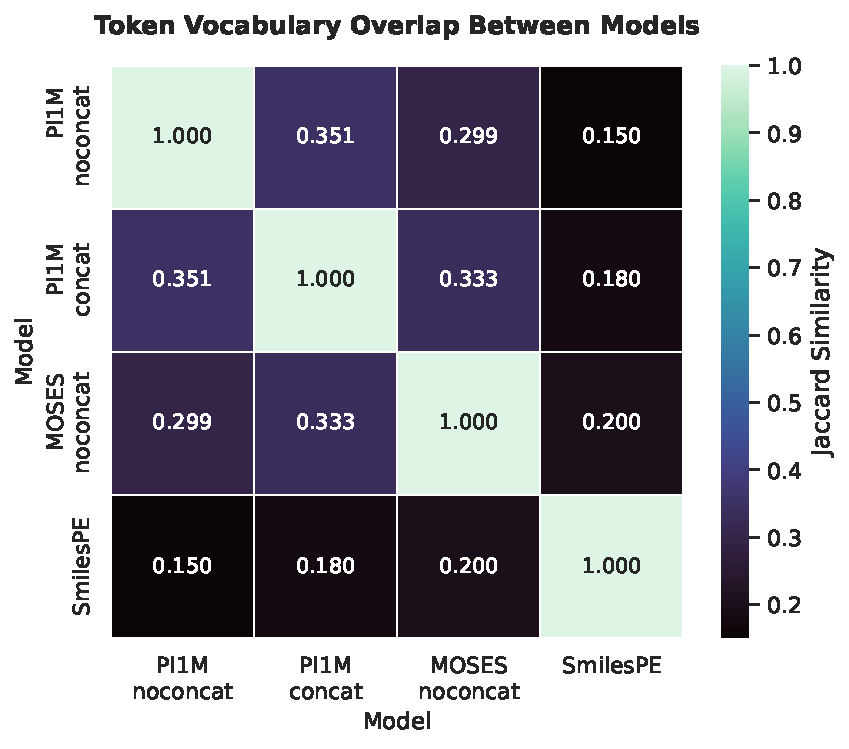
\includegraphics[width=\columnwidth]{figures/token_overlap_heatmap}}
\caption{Token vocabulary overlap (Jaccard similarity) between models. Polymer and molecular models share only 30\% of tokens, indicating dataset-specific vocabulary learning.}
\label{fig:overlap}
\end{center}
\vskip -0.2in
\end{figure}

Our central finding is that \hnet{} learns \emph{distinct tokenization strategies} for polymeric versus molecular SMILES. \Cref{tab:dataset_nature} quantifies this difference.

\begin{table}[t]
\caption{Comparison of polymer (PI1M) vs.\ molecular (MOSES) tokenization under matched conditions (340M bytes, no concatenation).}
\label{tab:dataset_nature}
\vskip 0.1in
\begin{center}
\begin{small}
\begin{tabular}{lcc}
\toprule
Metric & Value & Interpretation \\
\midrule
Token Overlap (Jaccard) & 0.30 & Distinct vocabularies \\
Breakpoint Overlap & 0.57 & Some shared motifs \\
KL Divergence & 3.92 & Large distribution gap \\
Tokens/SMILES (PI1M) & 22.0 & More complex \\
Tokens/SMILES (MOSES) & 18.5 & Simpler structures \\
\bottomrule
\end{tabular}
\end{small}
\end{center}
\vskip -0.1in
\end{table}

\begin{figure}[t]
  \vskip 0.1in
  \begin{center}
  \centerline{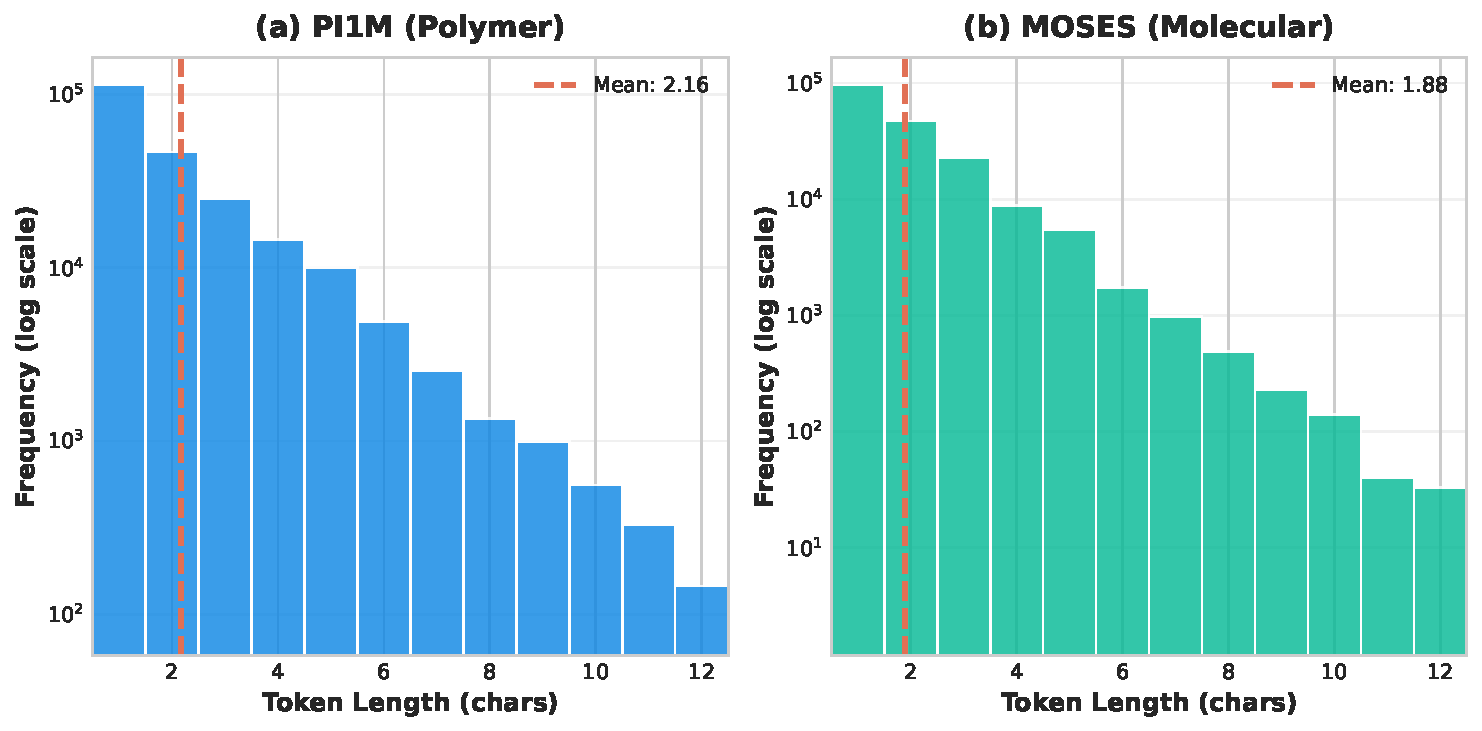
\includegraphics[width=\columnwidth]{figures/dataset_nature_token_lengths_noconcat}}
  \caption{Token length distributions for polymer (PI1M) and molecular (MOSES) datasets. Polymer tokenization produces shorter tokens (2.2 vs.\ 2.4 characters on average), reflecting finer-grained segmentation.}
  \label{fig:token_lengths}
  \end{center}
  \vskip -0.2in
  \end{figure}

Only 30\% of tokens are shared between polymer and molecular models (\cref{fig:overlap}), comparable to the divergence between language-specific models in NLP. The KL divergence of 3.92 indicates substantially different frequency distributions. Polymer SMILES consistently require $\sim$20\% more tokens, reflecting their inherent structural complexity. Notably, within-domain overlap (polymer models with different training settings) is only marginally higher at 35\%, suggesting that dataset nature is the dominant factor in vocabulary formation. Comparison with static \smilespe{} reveals even lower overlap: only 15--18\% with polymer models and $\sim$20\% with molecular models, underscoring that \hnet{} learns fundamentally different tokenization patterns than hand-designed chemical tokenizers. \Cref{fig:token_lengths} visualizes the token length distributions, showing that polymer tokenization produces shorter tokens on average (mean 2.2 vs.\ 1.9 characters), reflecting finer-grained segmentation adapted to the more complex polymeric structures.

Just as \hnet{} learns different tokens for Mandarin versus English~\citep{hwang2025hnet}, it discovers domain-specific ``chemical vocabularies''---byte patterns that efficiently represent polymer structures differ fundamentally from those optimal for drug-like molecules.

\subsection{Concatenation Effect}

Concatenating multiple SMILES during training provides longer context but could introduce noise from unrelated structures. \Cref{tab:concat} shows the effect.

\begin{table}[t]
\caption{Effect of concatenation (10$\times$ SMILES) on tokenization stability.}
\label{tab:concat}
\vskip 0.1in
\begin{center}
\begin{small}
\begin{tabular}{lccc}
\toprule
Dataset & Token Overlap & Breakpoint Stability & $\Delta$ Unique \\
\midrule
PI1M & 0.35 & 0.76 & +41\% \\
MOSES & 0.45 & \textbf{0.96} & +99\% \\
\bottomrule
\end{tabular}
\end{small}
\end{center}
\vskip -0.1in
\end{table}

Molecular SMILES show remarkable stability under concatenation---96\% of breakpoint positions are preserved, with 45\% token vocabulary overlap and a substantial 99\% increase in unique tokens discovered. Polymer SMILES show more variation (76\% breakpoint stability, 35\% token overlap, +41\% unique tokens), likely because their already-long sequences provide sufficient context even without concatenation.

Contrary to our initial hypothesis that polymers (being inherently concatenated structures) would be less affected, molecular SMILES actually showed greater stability. While the mechanism is not fully understood, one possibility is that the shorter, more stereotyped drug-like molecules have more consistent tokenization patterns that are robust to additional context.

\subsection{Scaling Behavior}

\begin{table}[t]
\caption{Effect of training compute on tokenization (PI1M, concatenated).}
\label{tab:training}
\vskip 0.1in
\begin{center}
\begin{small}
\begin{tabular}{lccccc}
\toprule
Bytes & FLOPs & Unique & Tok/SMILES & \bpb{} \\
\midrule
68M & 1.0e17 & 4,903 & 21.6 & 0.83 \\
340M & 5.0e17 & 5,775 & 18.2 & 0.69 \\
1.05B & 2.2e18 & 8,019 & 16.6 & \textbf{0.64} \\
\midrule
$\Delta$ & 22$\times$ & +63\% & $-$23\% & $-$23\% \\
\bottomrule
\end{tabular}
\end{small}
\end{center}
\vskip -0.1in
\end{table}

We examine how tokenization evolves with training using PI1M models at 68M, 340M, and 1.05B bytes processed (\cref{tab:training}). Extended training produces substantial improvements: 63\% more unique tokens, 23\% fewer tokens per SMILES (higher efficiency), and 30\% longer mean token length. Critically, breakpoint overlap between consecutive training stages remains high ($\geq$80\% agreement), reaching 91\% between 68M and 1.05B bytes models. This indicates that tokenization patterns stabilize quickly in early training, with later training refining \emph{what} tokens are learned while preserving \emph{where} boundaries occur. \Cref{app:evolution} visualizes this tokenization evolution during training, comparing 1-stage and 2-stage architectures on the same polymer SMILES across training checkpoints.

\textbf{Compression.} \bpb{} improves from 0.83 (68M bytes) to 0.64 (1.05B bytes), far better than random prediction (8.0) and comparable to well-trained English language models ($\sim$1.0--1.5 \bpb{}). This indicates \hnet{} learns meaningful chemical ``grammar''---predictable patterns in functional groups, rings, and stereochemistry.


\textbf{Scaling behavior.} We analyze how tokenization quality scales with training compute (\cref{tab:training}). \bpb{} improvement follows an approximate power law: \bpb{} $\propto$ FLOPs$^{-0.09}$ ($R^2 = 0.97$). Unique tokens increase 64\% with extended training, suggesting the model continues to discover specialized patterns rather than overfitting. Efficiency (tokens-per-SMILES) improves 23\% with diminishing returns, with most improvement in early training. These trends suggest that both larger models and longer training could further improve tokenization quality.

\subsection{Architecture: 1-Stage vs.\ 2-Stage}

The 2-stage architecture introduces hierarchical chunking with two levels of boundary prediction.

The 2-stage architecture provides only marginal compression improvement over the 1-stage variant: \bpb{} of 0.686 vs.\ 0.687 for PI1M (+0.2\%) and 0.679 vs.\ 0.682 for MOSES (+0.4\%)---differences that are not statistically significant. However, the hierarchical structure adds interpretability value by exposing tokenization at two levels: byte-to-chunk and chunk-to-superchunk groupings. This multi-scale view may prove useful for analyzing how models represent chemical hierarchies (e.g., atoms within functional groups within molecules), even if compression performance is similar. \Cref{app:evolution} shows the evolution of tokenization for both architectures. A detailed chemical interpretation of superchunk-level tokenization remains an avenue for future work, as our current analysis focuses primarily on the chunk level.

\subsection{H-Net vs.\ SmilesPE}


\begin{table}[t]
\caption{Comparison of tokenization approaches for chemical SMILES.}
\label{tab:benchmark}
\vskip 0.1in
\begin{center}
\begin{small}
\begin{tabular}{lcccc}
\toprule
 & \multicolumn{2}{c}{Tok Len} & \multicolumn{2}{c}{Tok/SMILES} \\
\cmidrule(lr){2-3} \cmidrule(lr){4-5}
Tokenizer & PI1M & MOSES & PI1M & MOSES \\
\midrule
Character & 1.0 & 1.0 & 48 & 35 \\
BPE & 3--4 & 3--4 & $\sim$14 & $\sim$10 \\
\smilespe{} & 4.2 & 5.9 & 11 & 6 \\
\hnet{} & 2.6 & 2.0 & 17 & 17 \\
\bottomrule
\end{tabular}
\end{small}
\end{center}
\vskip -0.1in
\end{table}

\Cref{tab:benchmark} compares \hnet{} against \smilespe{} and character-level baselines; \cref{app:benchmark} provides token length distributions. The three approaches represent fundamentally different tokenization philosophies with distinct trade-offs.

\textbf{Character-level} tokenization produces 48 tokens for polymer SMILES and 35 for molecular SMILES, providing no compression but maximum granularity. \textbf{\smilespe{}} achieves the best compression through chemistry-aware pair encoding pre-trained on ChEMBL, using longer tokens (4.2 characters for polymers, 5.9 for molecules) to reduce token counts to 11 and 6 respectively. \textbf{\hnet{}} occupies a middle ground: it produces more tokens than \smilespe{} (17 for both domains) but uses shorter, finer-grained tokens (2.6 characters for polymers, 2.0 for molecules).

Critically, \hnet{}'s tokenization is \emph{adaptive}: the vocabulary evolves with training data, enabling domain-specific patterns that static tokenizers cannot capture. While \smilespe{} uses the same pre-trained vocabulary regardless of whether it processes polymers or drug-like molecules, \hnet{} learns dataset-specific segmentation---discovering patterns like polymer attachment markers \texttt{[*]} or domain-specific functional groups. This adaptability is the key advantage: for downstream tasks requiring domain-specific chemical understanding, \hnet{}'s learned representations may provide better features than generic tokenization, as demonstrated in our property prediction results (\cref{sec:property}). Concrete tokenization examples are shown in \cref{app:examples}.

\subsection{Chemical Interpretability of Learned Tokens}

\begin{figure}[t]
\vskip 0.1in
\begin{center}
\centerline{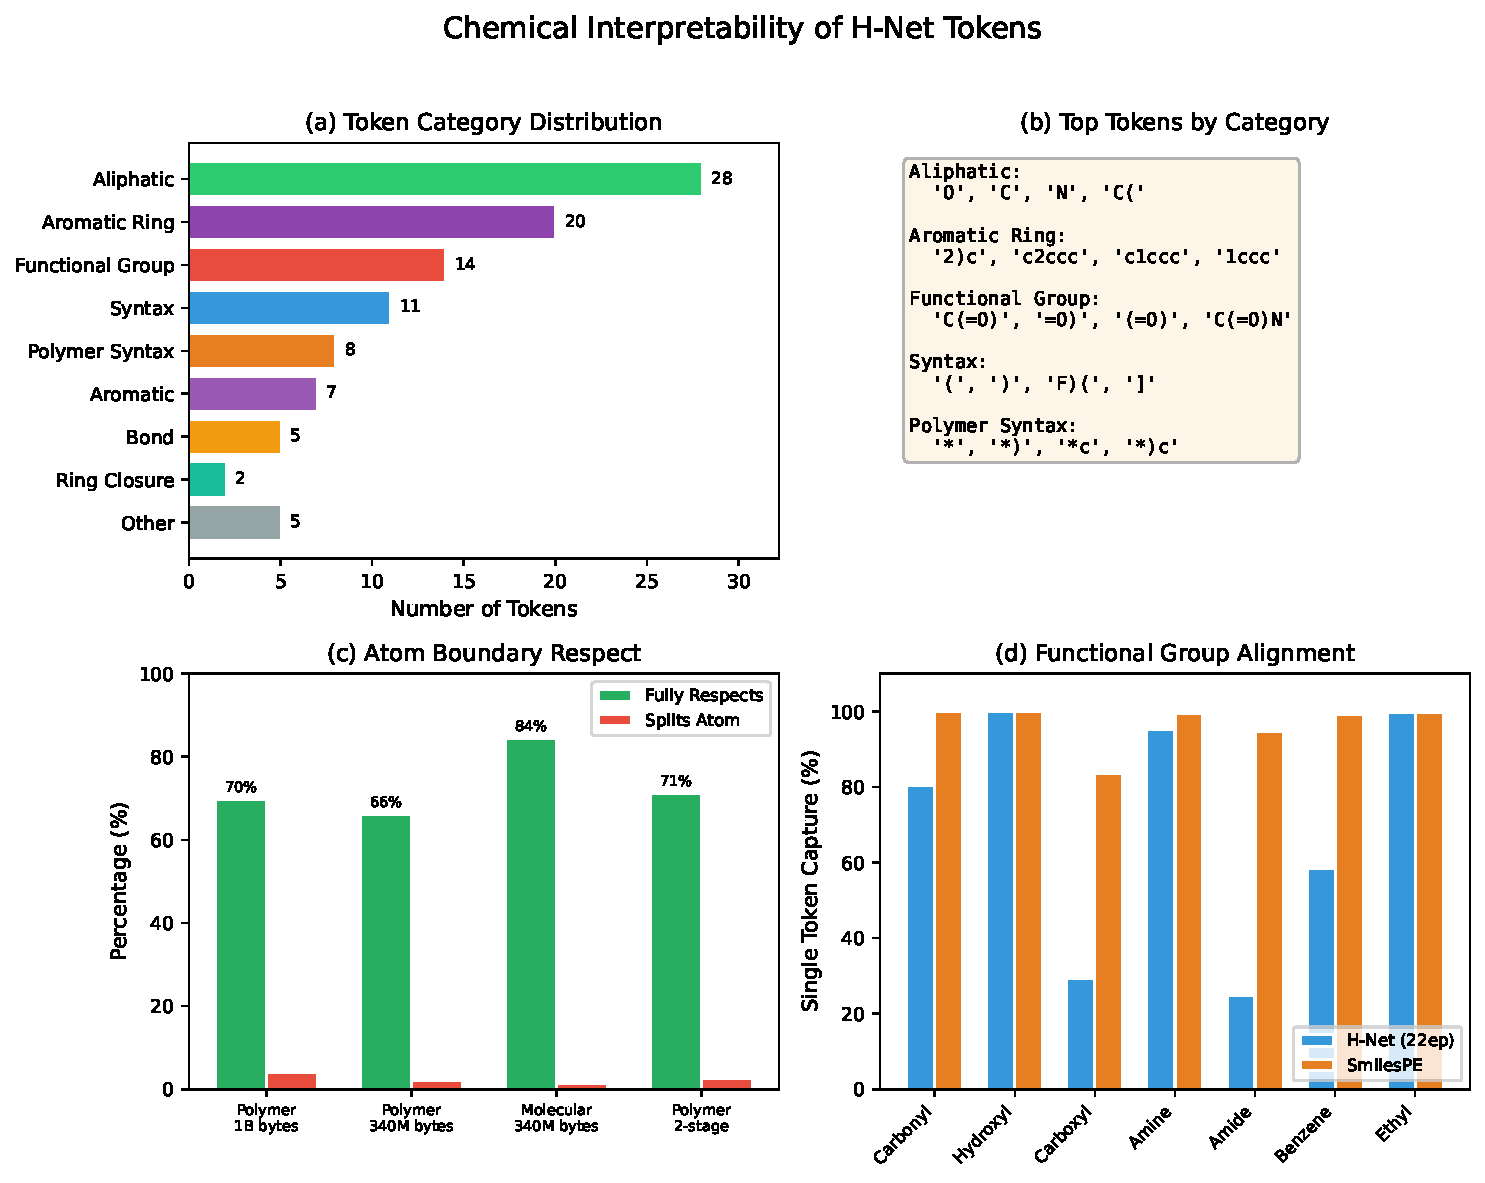
\includegraphics[width=\columnwidth]{figures/interpretability_analysis}}
\caption{Interpretability analysis of learned tokens. (a)~Token category distribution shows \hnet{} learns chemically meaningful patterns: aliphatic (28\%), aromatic (20\%), functional groups (14\%). (b)~Example tokens by category. (c)~Atom boundary respect rates across model variants. (d)~Functional group capture comparison between \hnet{} and \smilespe{}.}
\label{fig:interpretability}
\end{center}
\vskip -0.2in
\end{figure}

To understand what chemical patterns \hnet{} learns, we analyzed the top 100 most frequent tokens from our best-performing model (PI1M, 1.05B bytes). We automatically classified tokens using a hybrid approach combining character pattern heuristics, RDKit validation, and SMARTS functional group matching (\cref{fig:interpretability}).

\textbf{Token categories.} Aliphatic patterns constitute 28\% of frequent tokens, followed by aromatic rings (20\%), functional groups (14\%), and syntactic elements (11\%). This distribution suggests \hnet{} discovers chemically meaningful segmentation.

\textbf{Atom boundary respect.} In SMILES notation, atoms are represented by one or two characters (e.g., ``C'' for carbon, ``Cl'' for chlorine, ``Br'' for bromine). An ``atom boundary'' occurs between the end of one atom symbol and the start of the next; a tokenizer that ``respects'' atom boundaries never splits these multi-character symbols. Without any explicit chemical supervision, \hnet{} learns this property as an \emph{emergent behavior}: 70\% of tokens fully respect atom boundaries (both start and end on atom boundaries), while only 4\% split within an atom symbol (e.g., splitting ``Cl'' into ``C'' and ``l''). This emergent atomic awareness suggests that \hnet{}'s boundary prediction mechanism discovers fundamental chemical structure from raw byte sequences.

\textbf{Functional group alignment.} Functional groups are chemically meaningful substructures (e.g., hydroxyl -OH, carbonyl C=O, carboxyl -COOH) that determine molecular properties and reactivity. ``Functional group alignment'' measures whether a tokenizer captures these groups as single tokens rather than splitting them across multiple tokens. Simple groups like hydroxyl (-OH) and ethyl (-CC-) are captured as single tokens in $>$99\% of cases. Complex groups like carboxyl (-COOH) show lower alignment (25--30\%), as \hnet{} often splits these into multiple semantically meaningful pieces (e.g., ``C(=O)'' and ``O''). Unlike \smilespe{}'s chemically-derived vocabulary, \hnet{} discovers patterns bottom-up from data, trading some functional group alignment for dataset-specific patterns like polymer attachment markers (\texttt{[*]}).

%%%%%%%%%%%%%%%%%%%%%%%%%%%%%%%%%%%%%%%%%%%%%%%%%%%%%%%%%%%%%%%%%%%%%%%%%%%%%%%
\section{Application: Property Prediction}
\label{sec:property}
%%%%%%%%%%%%%%%%%%%%%%%%%%%%%%%%%%%%%%%%%%%%%%%%%%%%%%%%%%%%%%%%%%%%%%%%%%%%%%%

To validate that learned representations are useful, we evaluate \hnet{} embeddings for property prediction (\cref{tab:property}). We extract hidden state representations from the final Transformer layer before decoding, capturing the compressed latent space that encodes learned chemical structure. These 768-dimensional embeddings, obtained via mean pooling across all token positions, serve as molecular fingerprints. We then train XGBoost regressors and classifiers on these embeddings to predict chemical properties. This approach tests whether \hnet{}'s learned representations encode chemically relevant information transferable to downstream tasks. We compare against RDKit descriptors (2,248 dimensions total: Morgan fingerprints combined with 200 physicochemical descriptors), which are hand-engineered features based on explicit chemical knowledge rather than learned from data.

\begin{table}[t]
\caption{Property prediction results comparing \hnet{} embeddings vs.\ RDKit descriptors with XGBoost. H-Net uses 340M-byte 1-stage models: polymer model (PI1M-nocat) for Tg/MAC, molecular model (MOSES-nocat) for other tasks. Metrics: AUC = Area Under ROC Curve ($\uparrow$ higher is better), MAE = Mean Absolute Error ($\downarrow$ lower is better), RMSE = Root Mean Square Error ($\downarrow$ lower is better).}
\label{tab:property}
\vskip 0.1in
\begin{center}
\begin{small}
\begin{tabular}{llccc}
\toprule
Task & Metric & RDKit & \hnet{} & Model \\
\midrule
\multicolumn{5}{l}{\textit{Classification}} \\
BBBP & AUC$\uparrow$ & 0.927 & \textbf{0.950} & Mol. \\
HIV & AUC$\uparrow$ & 0.760 & \textbf{0.788} & Mol. \\
\midrule
\multicolumn{5}{l}{\textit{Regression}} \\
Tg & MAE$\downarrow$ & \textbf{24.8\textdegree{}C} & 26.6\textdegree{}C & Poly. \\
MAC & MAE$\downarrow$ & \textbf{5.7e-5} & 10.3e-5 & Poly. \\
Lipo. & MAE$\downarrow$ & \textbf{0.494} & 0.682 & Mol. \\
ESOL & RMSE$\downarrow$ & \textbf{0.660} & 0.910 & Mol. \\
FreeSolv & RMSE$\downarrow$ & \textbf{1.131} & 2.183 & Mol. \\
\bottomrule
\end{tabular}
\end{small}
\end{center}
\vskip -0.1in
\end{table}

Our extended evaluation across 7 benchmarks reveals a clear pattern. The benchmarks include: BBBP (Blood-Brain Barrier Penetration, 2K samples), HIV (HIV replication inhibition, 41K samples), Tg (polymer glass transition temperature), MAC (mass attenuation coefficient), Lipophilicity (octanol/water partition coefficient, 4.2K samples), ESOL (aqueous solubility, 1.1K samples), and FreeSolv (hydration free energy, 642 samples).

For \textbf{classification tasks}, \hnet{} consistently outperforms RDKit: on BBBP, \hnet{} achieves 0.950 AUC versus 0.927 for RDKit (+2.5\%); on the larger HIV dataset, the gap widens to +3.7\% (0.788 vs.\ 0.760), demonstrating that learned representations scale well to larger datasets. For \textbf{regression tasks}, RDKit outperforms across all benchmarks---Lipophilicity, ESOL, FreeSolv, MAC, and polymer Tg---suggesting that while \hnet{} captures high-level structural patterns relevant for classification, it misses the fine-grained quantitative features that traditional descriptors encode explicitly. Notably, \hnet{}'s polymer Tg prediction (26.6\textdegree{}C MAE) remains competitive with RDKit (24.8\textdegree{}C) and comparable to specialized methods like Lieconv-Tg~\citep{zhang2023lieconv}. Finally, mean pooling is essential: CLS-token pooling fails catastrophically, with AUC dropping 26\% on BBBP, indicating that chemical information is distributed across all token positions rather than concentrated in a single representation.

These results establish \hnet{} embeddings as complementary to traditional descriptors---excelling at classification where structural patterns drive decisions, while RDKit remains superior for regression requiring precise numerical features. \Cref{tab:property_full} provides detailed results across different \hnet{} model variants (varying training duration, architecture, and concatenation), showing relatively consistent performance across configurations---suggesting that \hnet{}'s representation quality is robust to hyperparameter choices.

Property prediction is not the primary focus of this work; rather, these experiments serve as a validation that \hnet{}'s learned tokenization produces chemically meaningful representations. The models used here were trained for tokenization analysis, not optimized for property prediction. Performance could likely be improved through task-specific fine-tuning, larger training corpora, or ensemble methods---directions we leave for future work. Our key contribution is demonstrating that dynamic tokenization produces useful chemical representations as a byproduct of learning to segment SMILES strings.

%%%%%%%%%%%%%%%%%%%%%%%%%%%%%%%%%%%%%%%%%%%%%%%%%%%%%%%%%%%%%%%%%%%%%%%%%%%%%%%
\section{Discussion}
\label{sec:discussion}
%%%%%%%%%%%%%%%%%%%%%%%%%%%%%%%%%%%%%%%%%%%%%%%%%%%%%%%%%%%%%%%%%%%%%%%%%%%%%%%

\textbf{Why does dynamic tokenization work?}
Chemical strings contain domain-specific patterns---functional groups, ring systems, stereochemistry markers---that benefit from adaptive segmentation. Static tokenizers impose uniform boundaries that may not align with chemical semantics, while \hnet{} discovers dataset-relevant patterns through end-to-end learning.

\textbf{Computational trade-offs.}
\hnet{}'s adaptive tokenization incurs computational cost. Training requires 18--72 hours on a single NVIDIA A10G GPU (24~GB) depending on training bytes (68M--1.05B), with peak memory usage of $\sim$18~GB. Inference achieves $\sim$1,000 SMILES/second on GPU with 15--20~GB memory. In contrast, \smilespe{} requires no training and achieves $\sim$50$\times$ higher throughput ($\sim$50,000 SMILES/sec on CPU) with minimal memory ($<$1~GB). This makes \smilespe{} more suitable for large-scale production pipelines, while \hnet{}'s investment is justified when dataset-specific tokenization provides tangible benefits for downstream tasks or interpretable domain-specific vocabulary. Following Sutton's Bitter Lesson~\citep{sutton2019bitter}, as computational costs continue to decline, learned approaches like \hnet{} that scale with data and compute will become increasingly practical---eventually making hand-designed tokenizers the exception rather than the rule.

\textbf{Cross-domain transfer.}
The 30\% token overlap between polymer and molecular vocabularies suggests significant degradation for cross-domain application. When a tokenizer trained on polymers is applied to drug-like molecules (or vice versa), the mismatched vocabulary forces fallback to shorter, less efficient tokens. Based on the vocabulary coverage, we estimate $\sim$50\% increase in tokens-per-SMILES for cross-domain tokenization, with corresponding BPB degradation. This validates our central finding: dataset-specific training captures domain patterns that generic tokenizers miss.

\textbf{Failure modes.}
Analysis of learned tokens reveals potential failure patterns: (1)~Atom symbol splitting, where two-letter symbols like Cl occasionally tokenize separately ($<$1\% of cases); (2)~Unbalanced brackets, where tokens contain partial parentheses representing meaningful subunits; (3)~Rare token overfitting, with $\sim$60\% of unique tokens appearing only once (hapax). These patterns suggest potential improvements through chemistry-aware boundary hints or curriculum learning. This should be investigated in future work.

%%%%%%%%%%%%%%%%%%%%%%%%%%%%%%%%%%%%%%%%%%%%%%%%%%%%%%%%%%%%%%%%%%%%%%%%%%%%%%%
\section{Conclusion}
\label{sec:conclusion}
%%%%%%%%%%%%%%%%%%%%%%%%%%%%%%%%%%%%%%%%%%%%%%%%%%%%%%%%%%%%%%%%%%%%%%%%%%%%%%%

We presented the first systematic study of dynamic tokenization for chemical SMILES using \hnet{}. Our key findings establish three main contributions. First, regarding \textbf{dataset specificity}, \hnet{} learns distinct tokenization strategies with only 30\% vocabulary overlap between polymer and molecular domains---a divergence comparable to that between different natural languages. Second, concerning \textbf{training dynamics}, extended training yields 63\% more unique tokens and 23\% higher efficiency without overfitting, demonstrating that the model continues to discover meaningful patterns rather than memorizing training data. Third, for \textbf{downstream performance}, \hnet{} embeddings outperform RDKit on classification benchmarks including BBBP (+2.5\% AUC) and HIV (+3.7\% AUC), demonstrating strong generalization across dataset scales from 2K to 41K samples, although property prediction should be studied further.

These results establish dynamic tokenization as a promising paradigm for chemical representation learning. Our findings support the principle articulated in Sutton's Bitter Lesson~\citep{sutton2019bitter}: learned approaches that scale with data and compute tend to outperform hand-engineered solutions. By removing fixed tokenization vocabularies, we enable models to discover optimal chemical segmentation directly from data.

Future work includes several promising directions. First, dynamic tokenization could be integrated as a preprocessing layer for existing chemical language models such as ChemBERTa~\citep{chithrananda2020chemberta} or MolGPT~\citep{bagal2021molegpt}, potentially combining the benefits of adaptive tokenization with the proven architectures of these models. Second, comparing \hnet{} embeddings against transformer-based chemical language models such as PolyBERT~\citep{kuenneth2023polybert} for property prediction would clarify relative strengths. Third, evaluating generative capabilities---using \hnet{} for molecular design and optimization---represents a natural extension of this work. Fourth, hybrid approaches could combine \hnet{}'s adaptability with chemistry-aware priors, guiding boundary prediction toward chemically meaningful segmentation. Fifth, extending the approach to other chemical string representations including XYZ coordinate files could broaden applicability. Finally, scaling to larger chemical corpora and model sizes may further improve tokenization quality, following the scaling trends we observe with training duration. Ultimately, as chemical datasets grow and compute becomes more accessible, learned tokenization offers a path toward chemical representations that continuously improve without manual vocabulary curation.

%%%%%%%%%%%%%%%%%%%%%%%%%%%%%%%%%%%%%%%%%%%%%%%%%%%%%%%%%%%%%%%%%%%%%%%%%%%%%%%
\section*{Impact Statement}
%%%%%%%%%%%%%%%%%%%%%%%%%%%%%%%%%%%%%%%%%%%%%%%%%%%%%%%%%%%%%%%%%%%%%%%%%%%%%%%

This paper presents work whose goal is to advance machine learning methods for chemical representation. Potential applications include drug discovery and materials design, which carry both benefits (accelerated therapeutic development) and risks (dual-use concerns). We encourage responsible deployment with appropriate safety considerations.

\section*{Code and Data Availability}

All code, trained models, and analysis scripts are publicly available at \url{https://anonymous.4open.science/r/hnet_smiles-2E43}. The repository includes training configurations, evaluation pipelines, and visualization tools to reproduce all results in this paper. The PI1M and MOSES datasets used for training are publicly available through their respective sources.

%%%%%%%%%%%%%%%%%%%%%%%%%%%%%%%%%%%%%%%%%%%%%%%%%%%%%%%%%%%%%%%%%%%%%%%%%%%%%%%
% References
%%%%%%%%%%%%%%%%%%%%%%%%%%%%%%%%%%%%%%%%%%%%%%%%%%%%%%%%%%%%%%%%%%%%%%%%%%%%%%%

\bibliography{references}
\bibliographystyle{icml2026}

%%%%%%%%%%%%%%%%%%%%%%%%%%%%%%%%%%%%%%%%%%%%%%%%%%%%%%%%%%%%%%%%%%%%%%%%%%%%%%%
% Appendix
%%%%%%%%%%%%%%%%%%%%%%%%%%%%%%%%%%%%%%%%%%%%%%%%%%%%%%%%%%%%%%%%%%%%%%%%%%%%%%%
\newpage
\appendix
\onecolumn

\section{Extended Results}
\label{app:results}

\subsection{Complete Model Comparison}

\begin{table}[h]
\caption{Complete tokenization statistics for all models.}
\label{tab:complete}
\begin{center}
\begin{tabular}{lcccccc}
\toprule
Model & Total Tokens & Unique Tokens & Tokens/SMILES & Mean Tok Len & \bpb{} & \ppl{} \\
\midrule
\multicolumn{7}{l}{\textit{PI1M (Polymer) Models}} \\
PI1M-1ep & 216,277 & 4,903 & 21.63 & 2.20 & 0.831 & 1.78 \\
PI1M-5ep & 182,298 & 5,775 & 18.23 & 2.62 & 0.687 & 1.61 \\
PI1M-22ep & 165,928 & 8,019 & 16.59 & 2.87 & 0.639 & 1.56 \\
PI1M-nocat & 220,423 & 4,094 & 22.04 & 2.17 & 0.670 & 1.59 \\
PI1M-2stg & 236,169 & 5,047 & 23.62 & 2.02 & 0.686 & 1.61 \\
\midrule
\multicolumn{7}{l}{\textit{MOSES (Molecular) Models}} \\
MOSES-5ep & 172,964 & 6,183 & 17.30 & 2.01 & 0.682 & 1.60 \\
MOSES-nocat & 184,614 & 3,112 & 18.46 & 2.12 & 0.658 & 1.58 \\
MOSES-2stg & 186,361 & 3,799 & 18.64 & 1.87 & 0.679 & 1.60 \\
\midrule
\multicolumn{7}{l}{\textit{SmilesPE Benchmark}} \\
SmilesPE-PI1M & 113,497 & 1,635 & 11.35 & 4.20 & --- & --- \\
SmilesPE-MOSES & 58,589 & 1,969 & 5.86 & 5.94 & --- & --- \\
\bottomrule
\end{tabular}
\end{center}
\end{table}


\subsection{Training Configurations}

All models were trained with the following configuration:
\begin{itemize}
    \item \textbf{Optimizer}: AdamW with weight decay 0.1
    \item \textbf{Learning rate}: $1 \times 10^{-4}$ base, with hierarchical modulation ($3\times$ for outer stages, $0.9\times$ for core network)
    \item \textbf{Batch size}: 64 per GPU step, gradient accumulation 8 (effective 512)
    \item \textbf{Precision}: bfloat16 mixed precision
    \item \textbf{Hardware}: Single NVIDIA A10G GPU (24 GB VRAM) on AWS EC2 g5.2xlarge instance
    \item \textbf{Training time}: 18--72 hours depending on training bytes (68M bytes $\approx$ 18 hours for PI1M)
    \item \textbf{Peak memory}: $\sim$18 GB GPU memory
\end{itemize}

\section{Tokenization Examples}
\label{app:examples}

\textbf{Example 1: Simple polymer}
\begin{verbatim}
PSMILES: [*]CC(=O)OCC[*]

H-Net tokens:  [*] | CC | (=O) | OCC | [*]
SmilesPE:      [*] | CC(=O)O | CC | [*]
\end{verbatim}

\textbf{Example 2: Drug-like molecule}
\begin{verbatim}
SMILES: CC(C)Cc1ccc(C(C)C(=O)O)cc1

H-Net tokens:  CC | (C) | Cc | 1 | ccc | (C | (C) | C(=O) | O) | cc | 1
SmilesPE:      CC(C) | Cc1ccc | (C(C) | C(=O)O) | cc1
\end{verbatim}

\section{Tokenization Evolution During Training}
\label{app:evolution}

\begin{figure}[h]
\begin{center}
\centerline{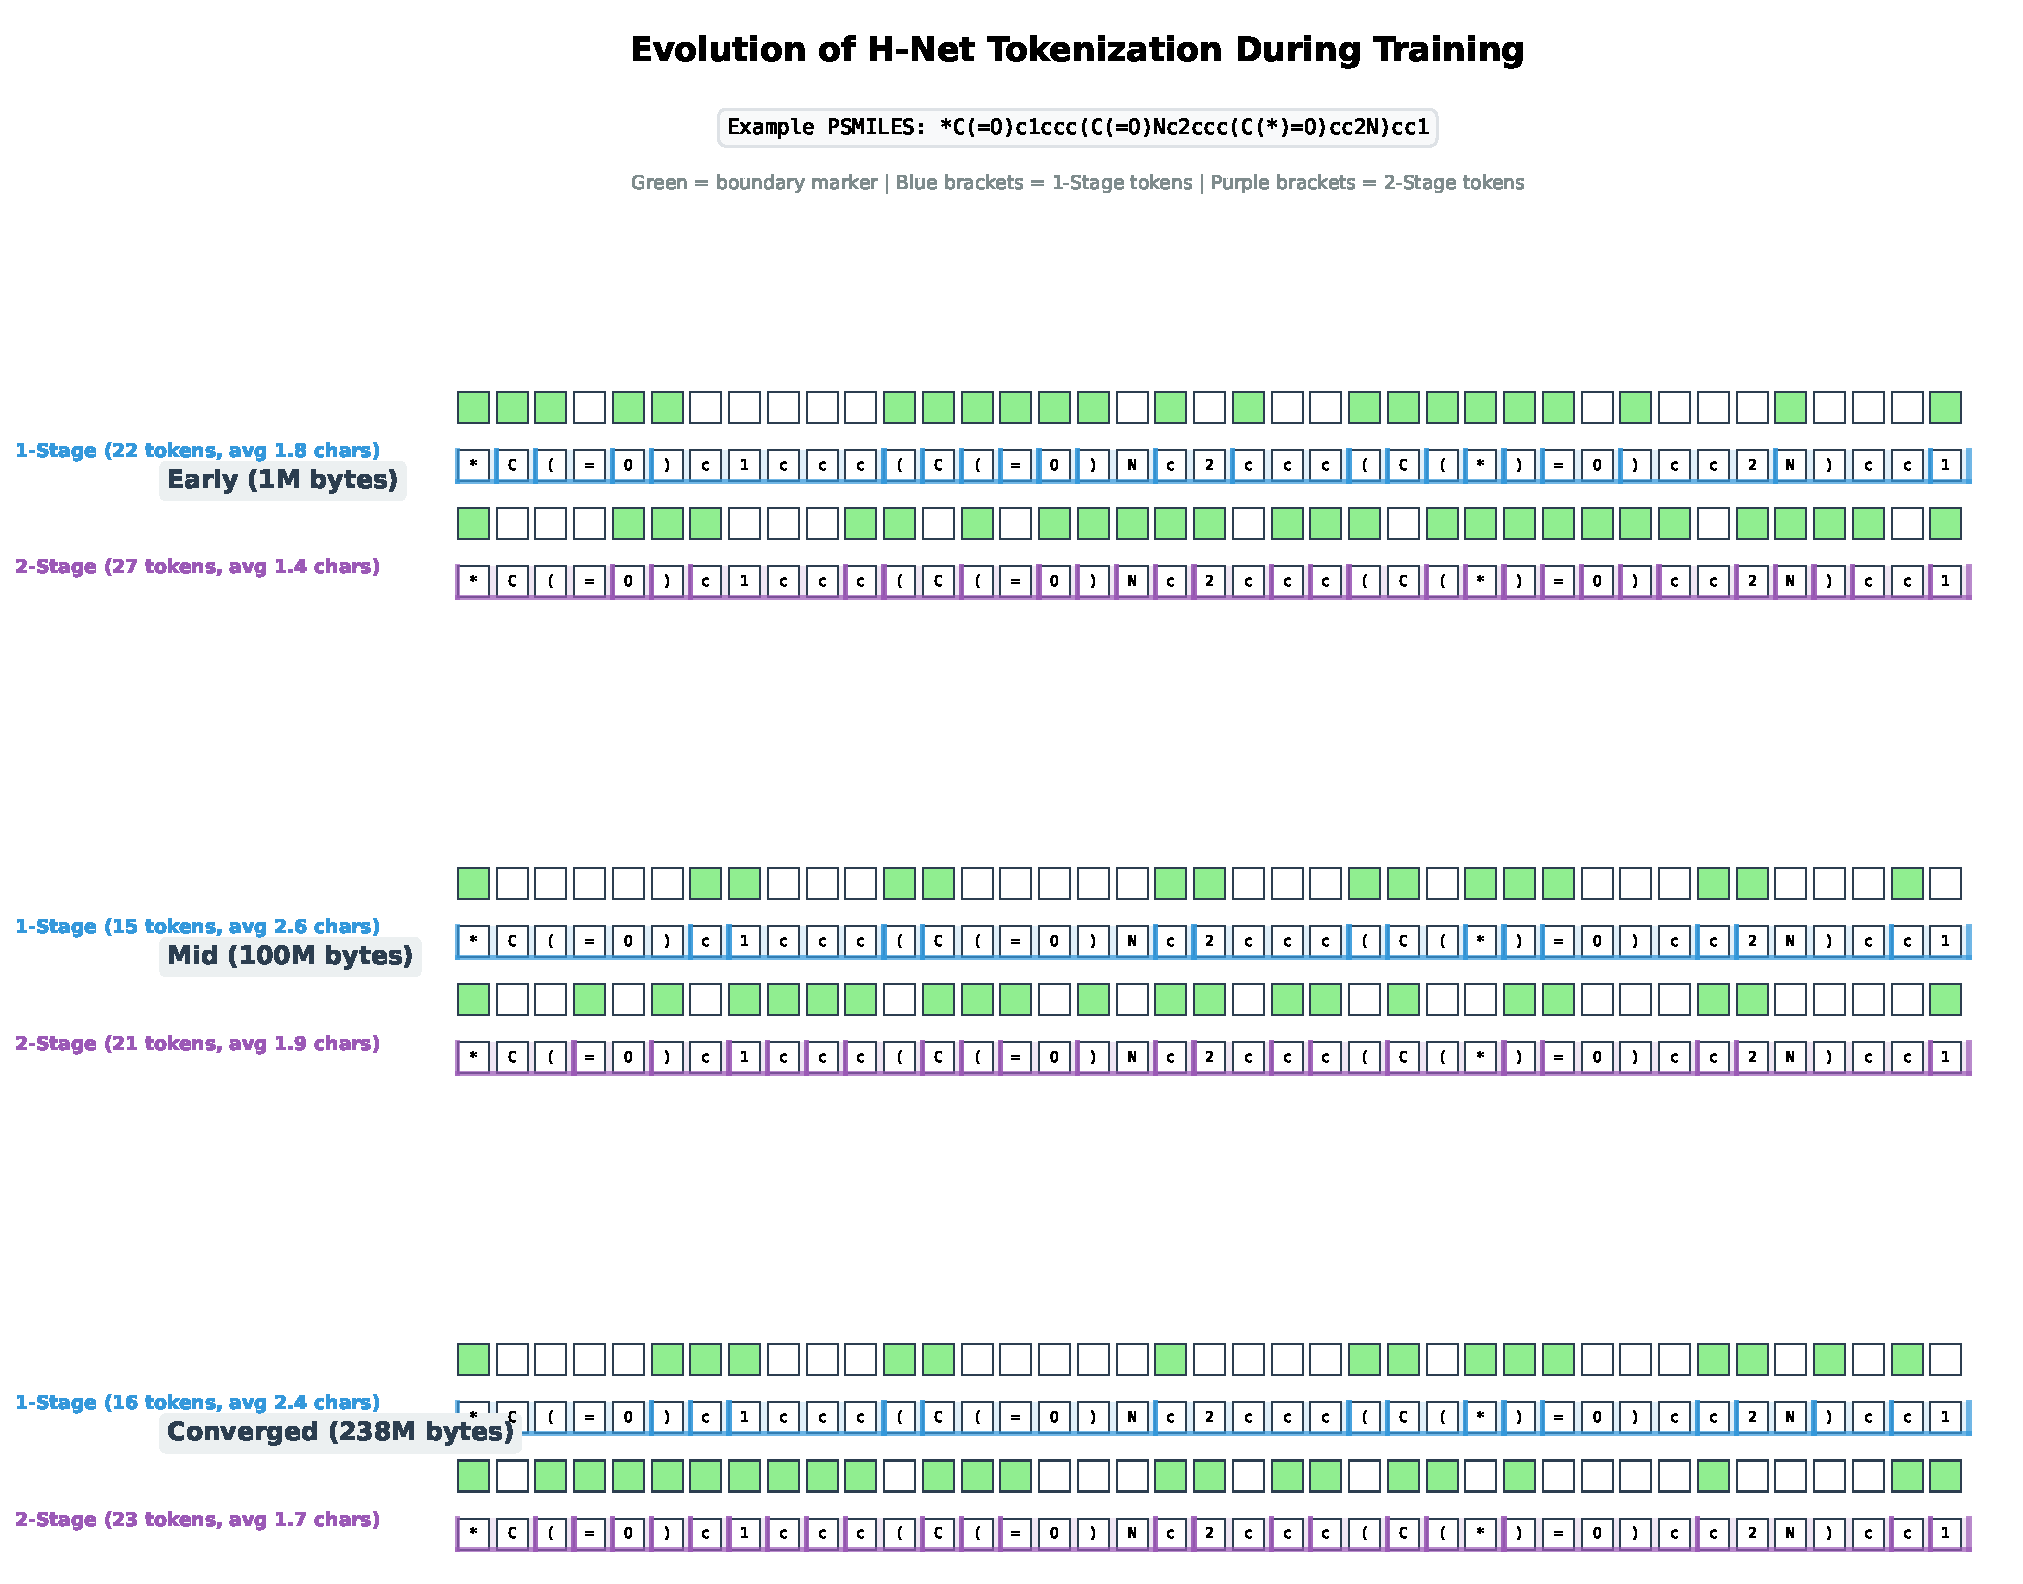
\includegraphics[width=0.9\textwidth]{figures/token_evolution_appendix}}
\caption{Evolution of H-Net tokenization during training, comparing 1-stage (blue) vs.\ 2-stage (purple) architecture on polymer SMILES (PI1M). Green squares indicate learned boundary positions; U-shape brackets show token spans. \textbf{Early training} (1M bytes): Both models produce near byte-level tokenization with many short tokens (1-stage: 22 tokens, 2-stage: 27 tokens). \textbf{Mid training} (100M bytes): The 1-stage model learns to group characters into chemical subunits, reducing to 15 tokens (avg 2.6 chars). \textbf{Converged} (238M bytes): Token patterns stabilize. The 1-stage architecture achieves better compression (16 tokens) compared to 2-stage (23 tokens), suggesting that for SMILES data the simpler architecture is more effective.}
\label{fig:token_evolution}
\end{center}
\end{figure}

The figure illustrates a key insight: as training progresses, H-Net learns to group bytes into chemically-meaningful units. Early in training, the boundary predictions are nearly random, producing byte-level tokenization. With more training, the model discovers patterns that correspond to chemical substructures---functional groups like carbonyl \texttt{(=O)}, aromatic rings \texttt{ccc}, and attachment points \texttt{[*]}.

Interestingly, the 1-stage architecture consistently outperforms the 2-stage variant on tokenization efficiency for SMILES data. This may be because chemical strings have relatively short-range dependencies compared to natural language, making hierarchical chunking less beneficial.

\section{Tokenizer Comparison}
\label{app:benchmark}

\begin{figure}[h]
\begin{center}
\centerline{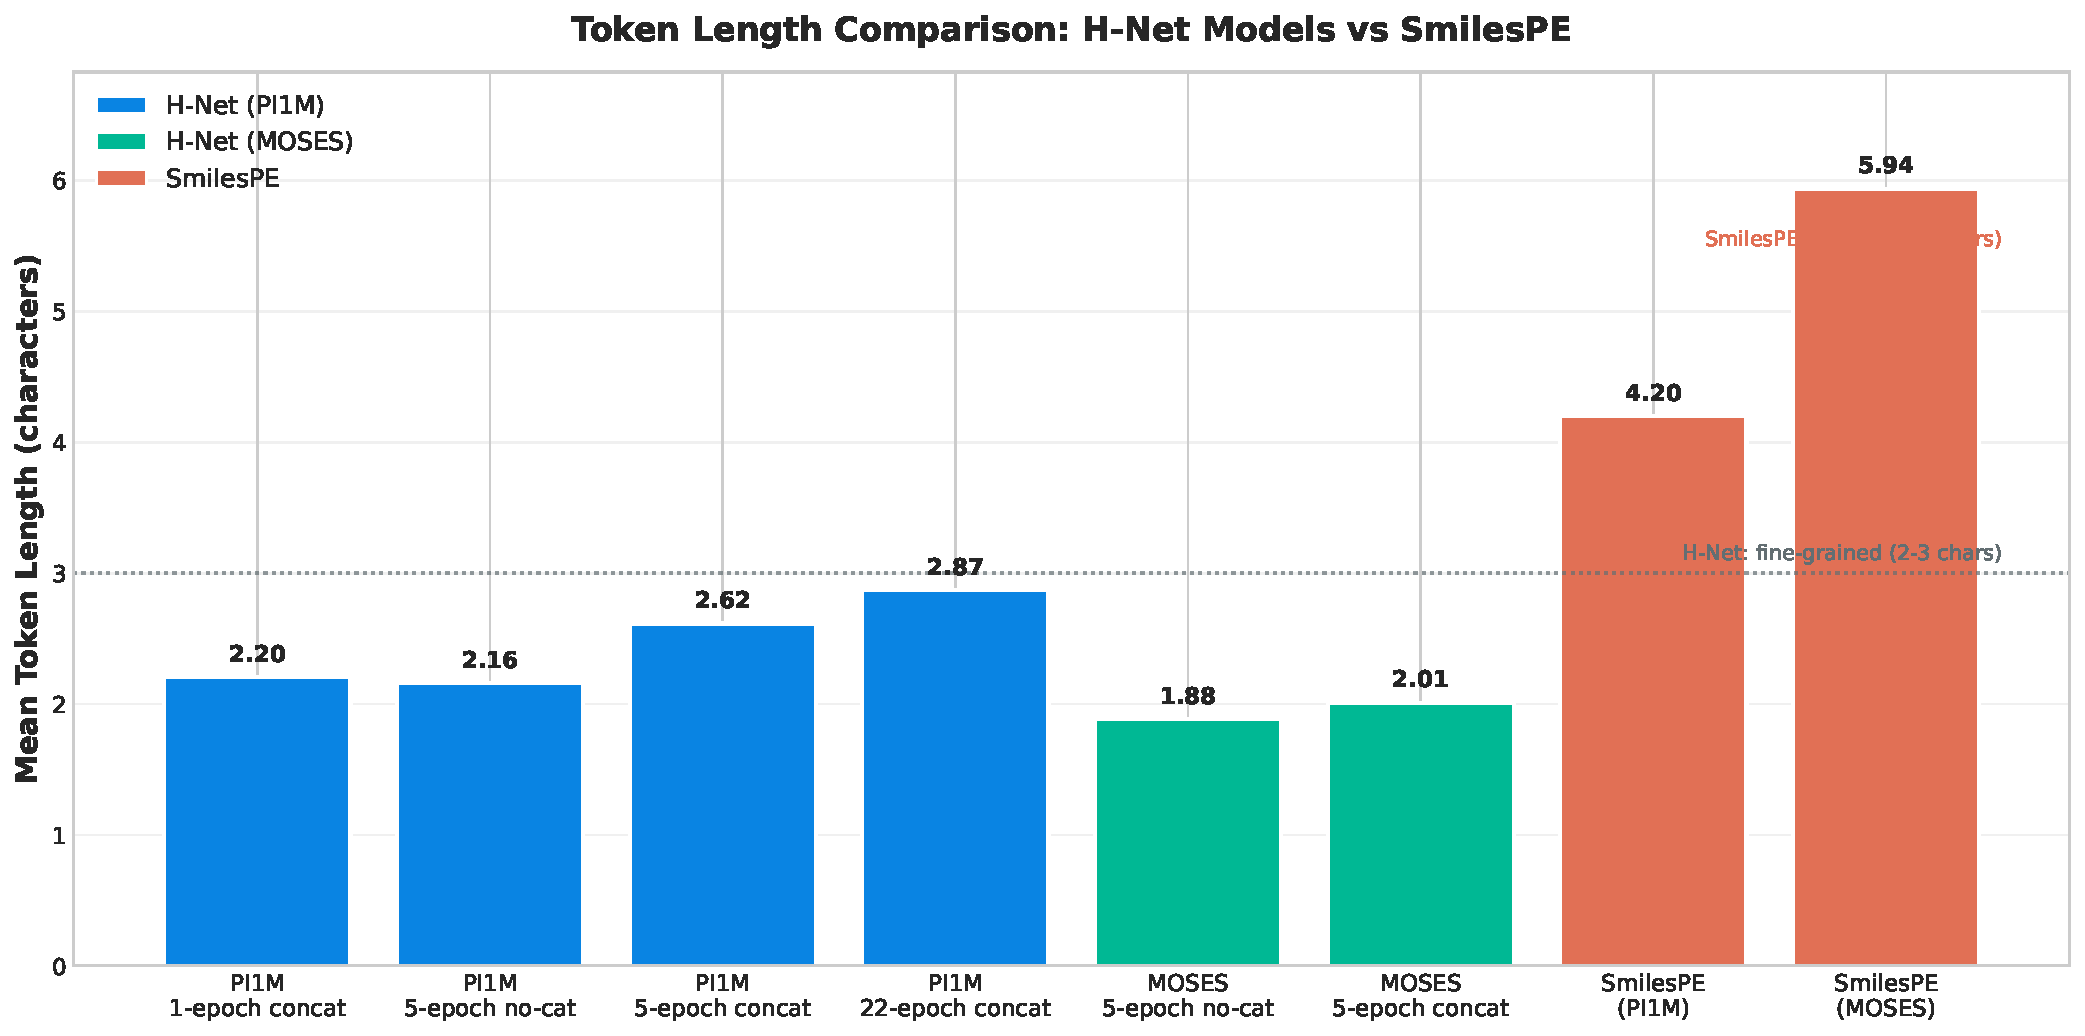
\includegraphics[width=0.7\textwidth]{figures/benchmark_token_lengths}}
\caption{Token length distributions comparing \hnet{} (2--3 characters) and \smilespe{} (4--6 characters). \hnet{} learns finer-grained, byte-level patterns while \smilespe{} uses coarser chemical subwords pre-trained on ChEMBL.}
\label{fig:benchmark_appendix}
\end{center}
\end{figure}

\section{Property Prediction Details}
\label{app:property}

\begin{table}[h]
\caption{Complete property prediction results comparing \hnet{} model variants. All results are 5-fold cross-validation with standard deviations. Tg and MAC use polymer-trained models; BBBP uses molecular-trained models. The table demonstrates that performance is relatively consistent across training configurations, with mean pooling essential for good results (CLS pooling fails catastrophically).}
\label{tab:property_full}
\begin{center}
\begin{tabular}{llccc}
\toprule
Model & Pooling & Tg MAE (\textdegree{}C) & MAC MAE & BBBP AUC \\
\midrule
RDKit & --- & 24.8 $\pm$ 0.7 & 5.7e-5 $\pm$ 0.2e-5 & 0.927 $\pm$ 0.009 \\
\midrule
hnet\_68M\_nocat & mean & 26.6 $\pm$ 0.6 & 10.3e-5 $\pm$ 0.3e-5 & --- \\
hnet\_340M\_nocat & mean & 27.0 $\pm$ 0.5 & 10.6e-5 $\pm$ 0.3e-5 & 0.950 $\pm$ 0.002 \\
hnet\_340M\_cat & mean & 26.9 $\pm$ 0.6 & 11.1e-5 $\pm$ 0.4e-5 & 0.949 $\pm$ 0.006 \\
hnet\_1B\_cat & mean & 28.2 $\pm$ 0.5 & 11.6e-5 $\pm$ 0.3e-5 & --- \\
hnet\_340M\_2stg & mean & 27.4 $\pm$ 0.8 & 11.4e-5 $\pm$ 0.3e-5 & 0.950 $\pm$ 0.009 \\
\midrule
hnet\_340M\_nocat & cls & 67.9 $\pm$ 1.3 & 26.0e-5 $\pm$ 0.4e-5 & 0.706 $\pm$ 0.024 \\
\bottomrule
\end{tabular}
\end{center}
\end{table}

\end{document}

